\section{Accomplishments}

\subsection{M\"obius Simulation}

\subsubsection{Failure Model}

In order to perform an effective failure analysis of the IlliniSat boot and recovery system, we first had to develop an error model to describe it.

We consider the IlliniSat system as failed if the system's Command and Data Handling (CD\&H) board is unable to resume normal operations after a fault occurs.  The satellite's health monitor already has support for a hardware watchdog timer; if the CD\&H board is unresponsive, it is assumed to have failed and it is rebooted \cite{jagannatha2014command}.  As such, the system is able to tolerate failure of the CD\&H system provided that the CD\&H board is able to boot the operating system and resume normal operation.  In this model, we consider the probability that this recovery process will not succeed as due to corruption of the operating system's image in flash memory.

This error model has two primary components: failures in RAM and the CD\&H system's execution that force a system reboot and failures in flash memory that prevent this reboot from being successful.  We only consider transient errors in this model.

We plan on modeling failures in flash memory as the interaction of two different cosmic ray-induced faults.  Single Event Upsets (SEUs) impact individual bits in memory and can be fixed with either active error correction or power-cycling.  Single Event Functional Interrupt (SEFI) events occur when the logic circuitry for the memory is hit, impacting normal operation.  We use the description of SEFIs in \cite{Gerardin2010Present} to guide our model; we assume that the flash memory is unresponsive after an SEFI until the memory is power-cycled.  

We plan on modeling failures in RAM as single-bit and page-wide errors, roughly following the results in \cite{Herrmann2013InSitu}.  We also assume that the CD\&H system experiences unspecified critical failures at some rate.

We assume that faults that affect a region of storage do so with equal probability across all address ranges; an image in RAM or in flash is corrupted if an fault affects any bits in its address range.

The literature seems to indicate that neither Single Event Latchup \cite{Langley2004SEE} or Total Ionizing Dose \cite{Likar2010Novel, Oldham2008TID, Herrmann2013InSitu} failure modes are likely for the given mission, so they are intentionally omitted here.

\subsubsection{M\"obius Baseline Model}

Using some of the parameters described in \cite{Oldham2008TID}, we have constructed a model in M\"obius to evaluate the reliability of the system without additional boot protection; this model will serve as a baseline reference for future experimentation.  The model is shown in more detail in Figure \ref{fig:ram} and \ref{fig:flash}.

\begin{figure}
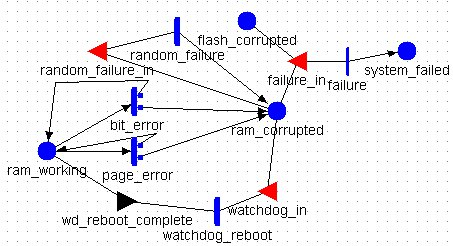
\includegraphics[width=0.5\textwidth]{ram_model}
\caption{The M\"obius model for the RAM subsystem.}
\label{fig:ram}
\end{figure}

\begin{figure}
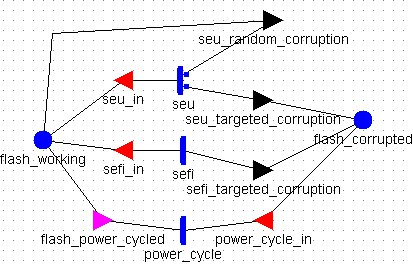
\includegraphics[width=0.5\textwidth]{flash_model}
\caption{The M\"obius model for the flash subsystem.}
\label{fig:flash}
\end{figure}


\subsection{Consistent Boot/Recovery Procedure}
The first challenge with this project was to get a working development
environment off the ground.  Installing QEMU was fairly straightforward, but
cross-compiling and getting u-boot and Linux to work took some effort.  We tried
a number of different ARM boards implemented in QEMU and eventually settled on
the ``versatilepb'' since it was the best documented.\footnote{http://balau82.wordpress.com/2010/03/10/u-boot-for-arm-on-qemu/}$^{,}$\footnote{http://elinux.org/Virtual\_Development\_Board}

After getting u-boot to work, we built a Linux kernel (version 3.2.67 was chosen
as IlliniSat is using a 3.2 based kernel) and booted that both with and without 
u-boot.  To demonstrate that the OS is working properly, we tried to get a
regular user process to run (by specifying it as the \fix{init} process).
However, this was highly non-trivial since it depended on things like system
call linkage, a working libc, and a filesystem.  Since the main project involves
the boot procedure, we will just boot the Linux kernel and let it panic by not
finding an init process. We intend to fix this for a proper demonstration in the
future.

It was discovered the u-boot has a built-in CRC-32 command, which we plan to
utilize. U-boot has two main ways of adding code: via scripts and standalone
applications.  After discovering to enable scripts (by modifying the
configuration header file), we have have decided to use the script method as
that is the most portable option. After properly configuring qemu and u-boot, we
have demonstrated the ability to get a working test script stored on a virtual
flash device.  This script modifies the u-boot environment and next we will work
on building the boot-assurance script.  


\subsection{Flash Patrol Read Daemon}
The Flash Patrol Read Daemon depends on being able to capture all file creations
and modifications in the filesystem. Supported by Linux 2.6.16 and after is an
API called \fix{inotify} that allows a user to monitor all filesystem events by
directory or by file using a user-specified watch list. Upon creation of the
\fix{inotify} instance, the user is able to interact with the instance using a
file descriptor. 

All of the events that happen on files tracked in the watch list are added to an
\fix{inotify} event buffer.  These events are then read and appropriate action
can be taken. For file creation and modification, we capture the event and then
create a file with ``\_crc'' appended to the name of the created/modified file.
Currently there are bugs with the CRC code, but this is where we will eventually
store the CRC value that is associated with the created/modified file.  If there
is enough free memory to support storing CRCs in memory (the IlliniSat team
expressed concerns with us storing too much state in memory), we can use the
same application and store them in \fix{tmpfs}.

We have also implemented this program as a daemon. The current na\"ive approach 
uses a polling method instead of signals.  By the final demonstration, this
will be changed so that the daemon does not use more resources.  It is undecided
if this should be part of the \fix{atd} scheduling employed by the C\&DH system
or separate.  We also intend to create a separate daemon that checks the CRC 
values on unmodified files to check for validity.  The challenge with this will
be the race condition on file modifications.  The first daemon would be
recalculating the CRC while the second daemon is checking the old CRC against
the new data.  A simple solution to this race condition would be to always run
them sequentially, but this may not be ideal from a power perspective.
